\section{Results and Discussion}
\label{sec:results}

\subsection{Convergence}

\lipsum[6]

% ── PNG figure (exported from a Python/matplotlib script in figures/) ─────────
\begin{figure}
  \centering
  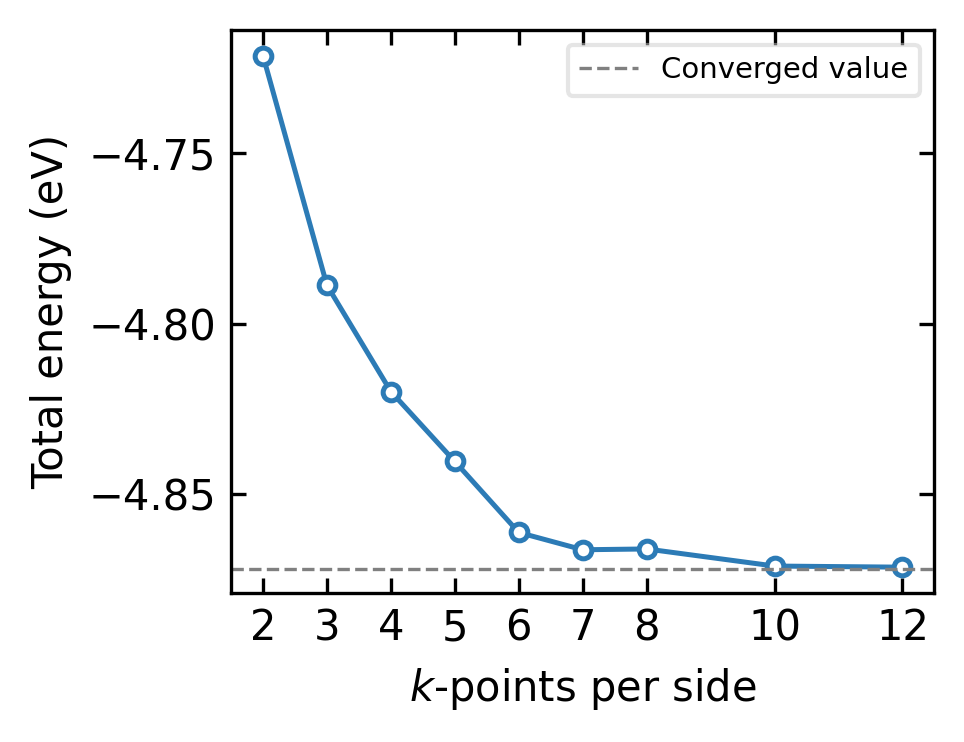
\includegraphics[width=\columnwidth]{figures/kpoint-convergence.png}
  \caption{%
    \textbf{$k$-point convergence.}
    Total energy as a function of $k$-points per side of the
    Monkhorst–Pack mesh.
    The dashed line marks the value used in all subsequent calculations.
  }
  \label{fig:kconv}
\end{figure}

\subsection{Main result}

\lipsum[7]

% ── pgfplots figure (data embedded directly — good for small datasets) ────────
\begin{figure}
  \centering
  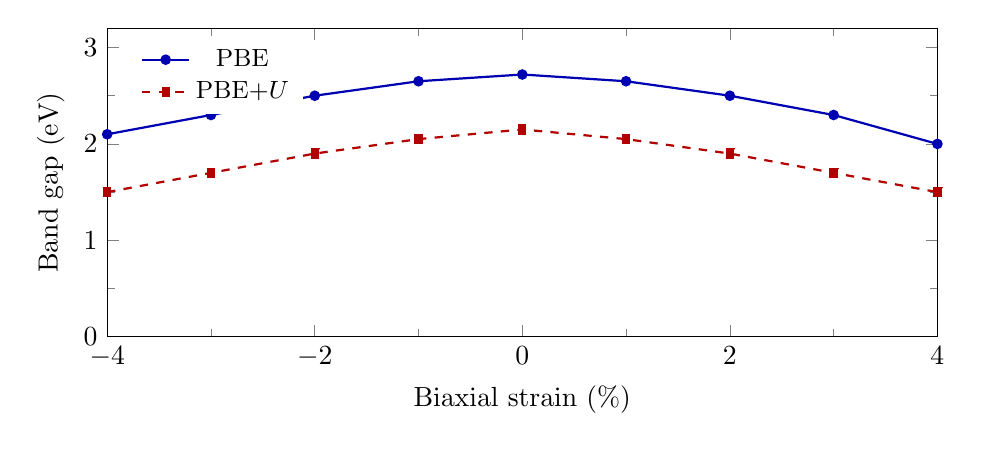
\begin{tikzpicture}
    \begin{axis}[
      width  = \columnwidth,
      height = 5.5cm,
      xlabel = {Biaxial strain (\%)},
      ylabel = {Band gap (eV)},
      xmin = -4, xmax = 4,
      ymin =  0, ymax = 3.2,
      xtick distance = 2,
      minor tick num  = 1,
      tick align = inside,
      axis line style = {thin},
      legend pos = north west,
      legend style = {font=\small, draw=none},
    ]
      \addplot[thick, color=blue!70!black, mark=*, mark size=1.5pt]
        coordinates {(-4,2.1)(-3,2.3)(-2,2.5)(-1,2.65)(0,2.72)(1,2.65)(2,2.5)(3,2.3)(4,2.0)};
      \addlegendentry{PBE}

      \addplot[thick, dashed, color=red!70!black, mark=square*, mark size=1.5pt]
        coordinates {(-4,1.5)(-3,1.7)(-2,1.9)(-1,2.05)(0,2.15)(1,2.05)(2,1.9)(3,1.7)(4,1.5)};
      \addlegendentry{PBE+$U$}
    \end{axis}
  \end{tikzpicture}
  \caption{%
    \textbf{Strain-tunable band gap.}
    Fundamental band gap as a function of biaxial strain.
    \todo{Replace with real data.}
  }
  \label{fig:pgf}
\end{figure}

\lipsum[8]
